\section{Verteilte Systeme}

\begin{definition}{Verteiltes System}\\
Ein Netzwerk aus autonomen Computern und Softwarekomponenten, die als einheitliches System erscheinen:
\begin{itemize}
    \item Autonome Knoten und Komponenten
    \item Netzwerkverbindung
    \item Erscheint als ein System
\end{itemize}
\end{definition}

\begin{concept}{Charakteristika verteilter Systeme}\\
Typische Merkmale moderner verteilter Systeme:
\begin{itemize}
    \item \textbf{Skalierbarkeit:} Oft sehr große Systeme
    \item \textbf{Datenorientierung:} Zentrale Datenbanken
    \item \textbf{Interaktivität:} GUI und Batch-Verarbeitung
    \item \textbf{Nebenläufigkeit:} Parallele Benutzerinteraktionen
    \item \textbf{Konsistenz:} Hohe Anforderungen an Datenkonsistenz
\end{itemize}
\end{concept}

\begin{theorem}{Grundlegende Konzepte}\\
\textbf{1. Kommunikation:}
\begin{itemize}
    \item Remote Procedure Calls (RPC)
    \item Message Queuing
    \item Publish-Subscribe-Systeme
\end{itemize}

\textbf{2. Fehlertoleranz:}
\begin{itemize}
    \item Replikation von Komponenten
    \item Failover-Mechanismen
    \item Fehlererkennung und -behandlung
\end{itemize}

\textbf{3. Fehlersemantik:}
\begin{itemize}
    \item Konsistenzgarantien
    \item Recovery-Verfahren
    \item Kompensationsmechanismen
\end{itemize}
\end{theorem}

\begin{concept}{Architekturmuster}\\
Grundlegende Architekturstile für verteilte Systeme:
\begin{itemize}
    \item \textbf{Client-Server:} Zentraler Server, multiple Clients
    \item \textbf{Peer-to-Peer:} Gleichberechtigte Knoten
    \item \textbf{Publish-Subscribe:} Event-basierte Kommunikation
\end{itemize}
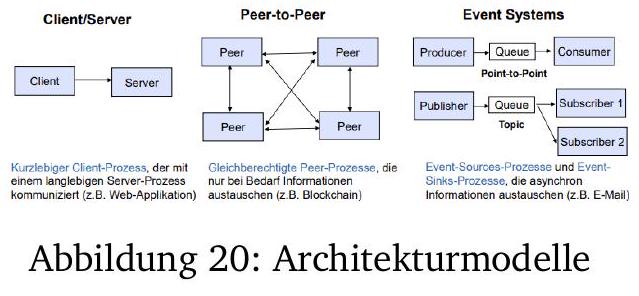
\includegraphics[width=0.9\linewidth]{images/2024_12_29_0d1d7b5551ea1b4b41bdg-18}
\end{concept}

\begin{example2}{Prüfungsaufgabe: Architekturstil-Analyse}
\textbf{Szenario:}
Ein Messaging-System soll entwickelt werden, das folgende Anforderungen erfüllt:
\begin{itemize}
    \item Hohe Skalierbarkeit
    \item Keine zentrale Komponente (Single Point of Failure)
    \item Direkter Nachrichtenaustausch zwischen Nutzern
    \item Offline-Fähigkeit
\end{itemize}

\textbf{Analysieren Sie die Architekturstile:}

\textbf{1. Client-Server}
\begin{itemize}
    \item \textbf{Vorteile:}
    \begin{itemize}
        \item Zentrale Verwaltung
        \item Einfache Konsistenzsicherung
    \end{itemize}
    \item \textbf{Nachteile:}
    \begin{itemize}
        \item Single Point of Failure
        \item Skalierungsprobleme
    \end{itemize}
\end{itemize}

\textbf{2. Peer-to-Peer}
\begin{itemize}
    \item \textbf{Vorteile:}
    \begin{itemize}
        \item Keine zentrale Komponente
        \item Direkte Kommunikation
        \item Gute Skalierbarkeit
    \end{itemize}
    \item \textbf{Nachteile:}
    \begin{itemize}
        \item Komplexe Konsistenzsicherung
        \item Schwierige Verwaltung
    \end{itemize}
\end{itemize}

\textbf{Empfehlung:} Peer-to-Peer mit hybriden Elementen
\end{example2}

\begin{KR}{Verteilungsprobleme analysieren}
\textbf{1. Probleme identifizieren}
\begin{itemize}
    \item \textbf{Netzwerk:}
    \begin{itemize}
        \item Latenz
        \item Bandbreite
        \item Ausfälle
    \end{itemize}
    \item \textbf{Daten:}
    \begin{itemize}
        \item Konsistenz
        \item Replikation
        \item Synchronisation
    \end{itemize}
    \item \textbf{System:}
    \begin{itemize}
        \item Skalierung
        \item Verfügbarkeit
        \item Wartbarkeit
    \end{itemize}
\end{itemize}

\textbf{2. Lösungsstrategien entwickeln}
\begin{itemize}
    \item \textbf{Netzwerk:}
    \begin{itemize}
        \item Caching
        \item Compression
        \item Redundanz
    \end{itemize}
    \item \textbf{Daten:}
    \begin{itemize}
        \item Eventual Consistency
        \item Master-Slave Replikation
        \item Konfliktauflösung
    \end{itemize}
    \item \textbf{System:}
    \begin{itemize}
        \item Load Balancing
        \item Service Discovery
        \item Circuit Breaker
    \end{itemize}
\end{itemize}
\end{KR}

\begin{example2}{Typische Prüfungsaufgabe: CAP-Theorem}
\textbf{Aufgabe:}
Analysieren Sie für ein verteiltes Datenbanksystem die Auswirkungen des CAP-Theorems.

\textbf{CAP-Theorem Komponenten:}
\begin{itemize}
    \item \textbf{Consistency:} Alle Knoten sehen dieselben Daten
    \item \textbf{Availability:} Jede Anfrage erhält eine Antwort
    \item \textbf{Partition Tolerance:} System funktioniert trotz Netzwerkausfällen
\end{itemize}

\textbf{Analyse der Trade-offs:}
\begin{itemize}
    \item \textbf{CA-System:}
    \begin{itemize}
        \item Hohe Konsistenz und Verfügbarkeit
        \item Keine Netzwerkpartitionierung möglich
        \item Beispiel: Traditionelle RDBMS
    \end{itemize}
    \item \textbf{CP-System:}
    \begin{itemize}
        \item Konsistenz und Partitionstoleranz
        \item Eingeschränkte Verfügbarkeit
        \item Beispiel: MongoDB
    \end{itemize}
    \item \textbf{AP-System:}
    \begin{itemize}
        \item Verfügbarkeit und Partitionstoleranz
        \item Eventual Consistency
        \item Beispiel: Cassandra
    \end{itemize}
\end{itemize}
\end{example2}

\begin{KR}{Verteilte System-Design}
\textbf{1. Anforderungsanalyse}
\begin{itemize}
    \item \textbf{Funktional:}
    \begin{itemize}
        \item Kernfunktionalitäten
        \item Datenmodell
        \item Schnittstellen
    \end{itemize}
    \item \textbf{Nicht-funktional:}
    \begin{itemize}
        \item Skalierbarkeit
        \item Verfügbarkeit
        \item Latenz
    \end{itemize}
\end{itemize}

\textbf{2. Architekturentscheidungen}
\begin{itemize}
    \item \textbf{Kommunikation:}
    \begin{itemize}
        \item Synchron vs. Asynchron
        \item Push vs. Pull
        \item Protokollwahl
    \end{itemize}
    \item \textbf{Datenmanagement:}
    \begin{itemize}
        \item Sharding
        \item Replikation
        \item Caching
    \end{itemize}
\end{itemize}

\textbf{3. Implementierungsaspekte}
\begin{itemize}
    \item \textbf{Fehlerbehandlung:}
    \begin{itemize}
        \item Retry-Strategien
        \item Fallbacks
        \item Monitoring
    \end{itemize}
    \item \textbf{Sicherheit:}
    \begin{itemize}
        \item Authentifizierung
        \item Verschlüsselung
        \item Autorisierung
    \end{itemize}
\end{itemize}
\end{KR}

\begin{KR}{Entwurf verteilter Systeme}\\
\textbf{1. Systemanalyse}
\begin{itemize}
    \item Anforderungen identifizieren
    \item Verteilungsaspekte analysieren
    \item Konsistenzanforderungen definieren
\end{itemize}

\textbf{2. Architekturentscheidungen}
\begin{itemize}
    \item Architekturstil wählen
    \item Kommunikationsmuster festlegen
    \item Fehlertoleranzstrategie definieren
\end{itemize}

\textbf{3. Technologieauswahl}
\begin{itemize}
    \item Middleware evaluieren
    \item Protokolle bestimmen
    \item Werkzeuge auswählen
\end{itemize}
\end{KR}

\begin{concept}{Middleware-Technologien}\\
Gängige Technologien für verteilte Systeme:
\begin{itemize}
    \item \textbf{Message Broker:} 
    \begin{itemize}
        \item Apache Kafka
        \item RabbitMQ
    \end{itemize}
    \item \textbf{RPC Frameworks:}
    \begin{itemize}
        \item gRPC
        \item CORBA
    \end{itemize}
    \item \textbf{Web Services:}
    \begin{itemize}
        \item RESTful APIs
        \item GraphQL
    \end{itemize}
\end{itemize}
\end{concept}



\begin{KR}{Typische Fehlerquellen}\\
\textbf{1. Netzwerkfehler}
\begin{itemize}
    \item Verbindungsabbrüche
    \item Timeouts
    \item Partitionierung
\end{itemize}

\textbf{2. Konsistenzprobleme}
\begin{itemize}
    \item Race Conditions
    \item Veraltete Daten
    \item Lost Updates
\end{itemize}

\textbf{3. Skalierungsprobleme}
\begin{itemize}
    \item Lastverteilung
    \item Resource-Management
    \item Bottlenecks
\end{itemize}

\textbf{Lösungsstrategien:}
\begin{itemize}
    \item Circuit Breaker Pattern
    \item Retry mit Exponential Backoff
    \item Idempotente Operationen
    \item Optimistic Locking
\end{itemize}
\end{KR}

